% Asset ID: AS1GraphsTransformationsTikZ-001
% Source: CCEA AS1-AF-LO012 + DrFrost Chapter 4 cubic graph evidence
% Related lesson section: Core Theory and Worked Example 1
% Purpose: Sketch y=(x-2)(1-x)(1+x), showing roots and y-intercept
\documentclass[tikz,border=8pt]{standalone}
\usepackage{pgfplots}
\pgfplotsset{compat=1.18}
\begin{document}
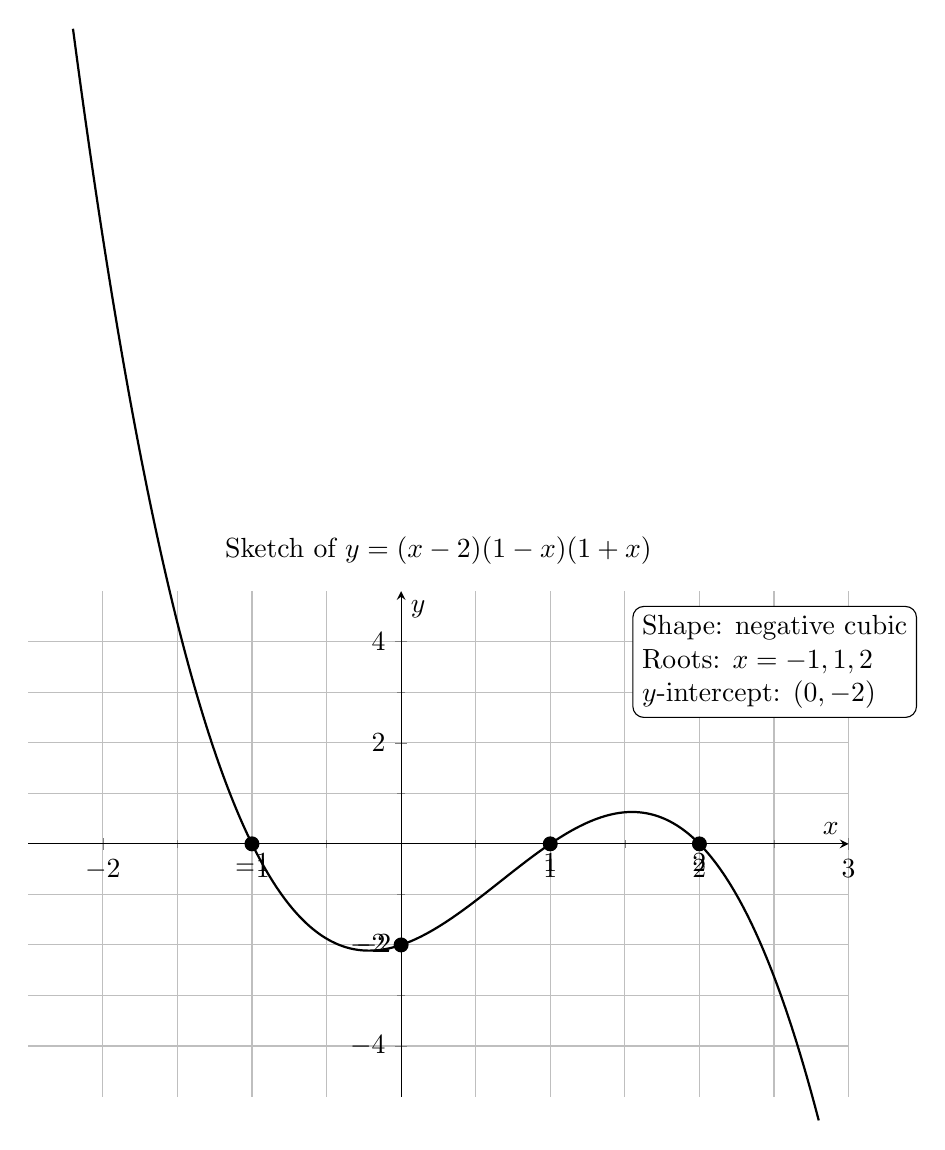
\begin{tikzpicture}
\begin{axis}[axis lines=middle,xmin=-2.5,xmax=3,ymin=-5,ymax=5,xlabel={$x$},ylabel={$y$},xtick={-2,-1,0,1,2,3},ytick={-4,-2,0,2,4},grid=both,minor tick num=1,width=12cm,height=8cm,samples=200,domain=-2.2:2.8,enlargelimits=false,clip=false,title={Sketch of $y=(x-2)(1-x)(1+x)$}]
\addplot[thick,smooth]{(x-2)*(1-x)*(1+x)};
\addplot[only marks,mark=*,mark size=2.5pt] coordinates {(-1,0) (1,0) (2,0)};
\addplot[only marks,mark=*,mark size=2.5pt] coordinates {(0,-2)};
\node[anchor=north] at (axis cs:-1,0) {$-1$};
\node[anchor=north] at (axis cs:1,0) {$1$};
\node[anchor=north] at (axis cs:2,0) {$2$};
\node[anchor=east] at (axis cs:0,-2) {$-2$};
\node[draw,rounded corners,fill=white,align=left,anchor=west] at (axis cs:1.55,3.6){Shape: negative cubic\\Roots: $x=-1,1,2$\\$y$-intercept: $(0,-2)$};
\end{axis}
\end{tikzpicture}
\end{document}
